\documentclass[12pt,a4paper]{article}

\usepackage{amsmath}
\usepackage{amssymb}
\pagestyle{empty}
\usepackage[margin=1in]{geometry}
\usepackage{hyperref}
\usepackage[utf8]{inputenc}
\usepackage[IL2]{fontenc}
\usepackage[czech]{babel}
\usepackage{amsthm}
\usepackage{enumitem}
\usepackage{graphicx}

\theoremstyle{definition}
\newtheorem{uloha}{Úloha}
\newtheorem*{bonus}{Bonus}

\DeclareMathOperator{\tg}{tg}
\def\ee{\mathrm{e}}

\setlist[enumerate]{label={(\alph*)}}

\begin{document}

\section*{Derivace -- test na monotónnost a extrémy}
%\bigskip

%\emph{Výsledky jsou na druhé straně.}

%Zderivujte uvedené funkce. V mnoha případech je možné nejprve výraz trochu upravit, čímž si člověk zjednoduší derivování, případně využít toho, co už má spočtené.
\begin{uloha}
Určete rovnici tečny %k funkci
ke grafu funkce $f(x) = \dfrac{x+1}{x+2}$ v bodě $-1$.
%\begin{enumerate}
	%\item k funkci $2^x$ v bodě $0$,
	%\item k funkci $\sin x$ v bodě $\pi$.
%\end{enumerate}
\end{uloha}


\begin{uloha}
U následujících funkcí určete maximální (tj. co největší) intervaly, na kterých je funkce rostoucí či klesající, a nalezněte všechna lokální maxima a minima.
\begin{enumerate}
	\item $g_a(x) = 2x + \dfrac{1}{x^2}$
	\item $g_b(x) = -3x^4 + 16x^3 - 24x^2 + 12$
	\item $g_c(x) = x \cdot \ee^{-x^2}$
\end{enumerate}
\end{uloha}


\begin{uloha}
Nalezněte globální extrémy funkce 
	$h(x) = \ln(x^2 + 1)$  na intervalu $\langle-1; 2\rangle$.
%\end{enumerate}
\end{uloha}


\begin{bonus}[za 1 bod]
\uv{Rozstříhejte} čtverec $9 \times 9$ níže na deset čtverců tak, abyste dostali aspoň jeden čtverec $1 \times 1$, aspoň jeden čtverec $2 \times 2$, aspoň jeden čtverec $3 \times 3$, aspoň jeden čtverec $4 \times 4$ a aspoň jeden čtverec $5 \times 5$.
\[ 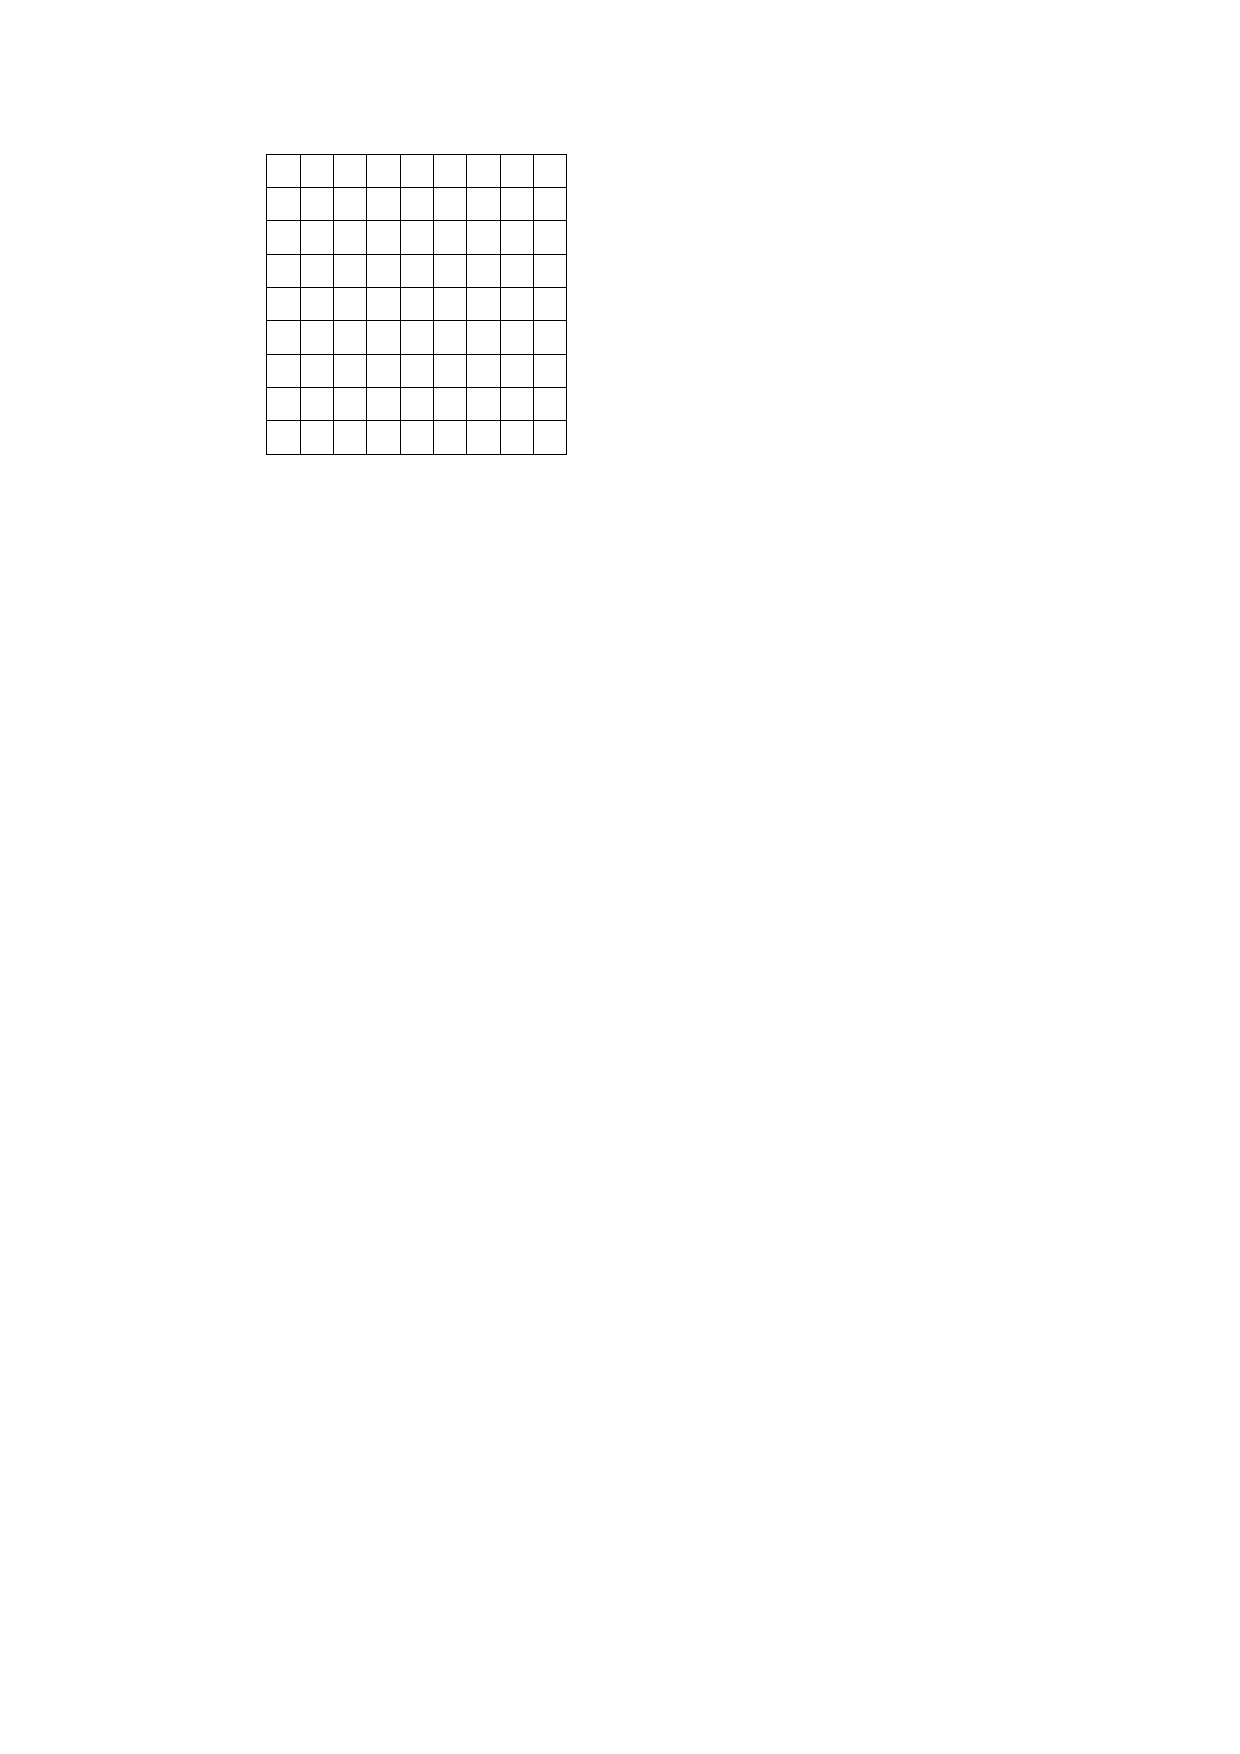
\includegraphics[scale=.8]{mrizka.pdf} \]
\end{bonus}


\end{document}